\documentclass[paper=letter,11pt]{scrartcl}

\KOMAoptions{headinclude=true, footinclude=false}
\KOMAoptions{DIV=14, BCOR=5mm}
\KOMAoptions{numbers=noendperiod}
\KOMAoptions{parskip=half}
\addtokomafont{disposition}{\rmfamily}
\addtokomafont{part}{\LARGE}
\addtokomafont{descriptionlabel}{\rmfamily}
%\setkomafont{pageheadfoot}{\normalsize\sffamily}
\setkomafont{pagehead}{\normalsize\rmfamily}
%\setkomafont{publishers}{\normalsize\rmfamily}
\setkomafont{caption}{\normalfont\small}
\setcapindent{0pt}
\deffootnote[1em]{1em}{1em}{\textsuperscript{\thefootnotemark}\ }


\usepackage{amsmath}
\usepackage[varg]{txfonts}
\usepackage[T1]{fontenc}
\usepackage{graphicx}
\usepackage{xcolor}
\usepackage[american]{babel}
% hyperref is needed in many places, so include it here
\usepackage{hyperref}

\usepackage{xspace}
\usepackage{multirow}
\usepackage{float}


\usepackage{braket}
\usepackage{bbm}
\usepackage{relsize}
\usepackage{tcolorbox}

\def\ketY{\ensuremath{\ket {\Psi}}}
\def\iGeV{\ensuremath{\textrm{GeV}^{-1}}}
%\def\mp{\ensuremath{m_{\textrm{proton}}}}
\def\rp{\ensuremath{r_{\textrm{proton}}}}
\def\me{\ensuremath{m_{\textrm{electron}}}}
\def\aG{\ensuremath{\alpha_G}}
\def\rAtom{\ensuremath{r_{\textrm{atom}}}}
\def\rNucl{\ensuremath{r_{\textrm{nucleus}}}}
\def\GN{\ensuremath{\textrm{G}_\textrm{N}}}
\def\ketX{\ensuremath{\ket{\vec{x}}}}
\def\ve{\ensuremath{\vec{\epsilon}}}


\def\ABCDMatrix{\ensuremath{\begin{pmatrix} A &  B  \\ C  & D \end{pmatrix}}}
\def\xyprime{\ensuremath{\begin{pmatrix} x' \\ y' \end{pmatrix}}}
\def\xyprimeT{\ensuremath{\begin{pmatrix} x' &  y' \end{pmatrix}}}
\def\xy{\ensuremath{\begin{pmatrix} x \\ y \end{pmatrix}}}
\def\xyT{\ensuremath{\begin{pmatrix} x & y \end{pmatrix}}}

\def\IMatrix{\ensuremath{\begin{pmatrix} 0 &  1  \\ -1  & 0 \end{pmatrix}}}
\def\IBoostMatrix{\ensuremath{\begin{pmatrix} 0 &  1  \\ 1  & 0 \end{pmatrix}}}
\def\JThree{\ensuremath{\begin{pmatrix}    0 & -i & 0  \\ i & 0  & 0 \\ 0 & 0 & 0 \end{pmatrix}}} 
\def\JTwo{\ensuremath{\begin{bmatrix}    0 & 0 & -i  \\ 0 & 0  & 0 \\ i & 0 & 0 \end{bmatrix}}}
\def\JOne{\ensuremath{\begin{bmatrix}    0 & 0 & 0  \\ 0 & 0  & -i \\ 0 & i & 0 \end{bmatrix}}}
\def\etamn{\ensuremath{\eta_{\mu\nu}}}
\def\Lmn{\ensuremath{\Lambda^\mu_\nu}}
\def\dmn{\ensuremath{\delta^\mu_\nu}}
\def\wmn{\ensuremath{\omega^\mu_\nu}}
\def\be{\begin{equation*}}
\def\ee{\end{equation*}}
\def\bea{\begin{eqnarray*}}
\def\eea{\end{eqnarray*}}
\def\bi{\begin{itemize}}
\def\ei{\end{itemize}}
\def\fmn{\ensuremath{F_{\mu\nu}}}
\def\fMN{\ensuremath{F^{\mu\nu}}}
\def\bc{\begin{center}}
\def\ec{\end{center}}
\def\nus{$\nu$s}

\def\adagger{\ensuremath{a_{p\sigma}^\dagger}}
\def\lineacross{\noindent\rule{\textwidth}{1pt}}

\newcommand{\multiline}[1] {
\begin{tabular} {|l}
#1
\end{tabular}
}

\newcommand{\multilineNoLine}[1] {
\begin{tabular} {l}
#1
\end{tabular}
}



\newcommand{\lineTwo}[2] {
\begin{tabular} {|l}
#1 \\
#2
\end{tabular}
}

\newcommand{\rmt}[1] {
\textrm{#1}
}


%
% Units
%
\def\m{\ensuremath{\rmt{m}}}
\def\GeV{\ensuremath{\rmt{GeV}}}
\def\pt{\ensuremath{p_\rmt{T}}}


\def\parity{\ensuremath{\mathcal{P}}}

\usepackage{cancel}
\usepackage{ mathrsfs }
\def\bigL{\ensuremath{\mathscr{L}}}

\usepackage{ dsfont }



\usepackage{fancyhdr}
\fancyhf{}

%\documentclass[margin,line]{res}
\usepackage{braket}

\def\ketY{\ensuremath{\ket {\Psi}}}

\begin{document}

\section{What this course is really about:}
The course Title is: Introduction to Particle Physics.
Technically correct, misses general philosophy. 
We are interested in how the world works. 
Turns out, one major lesson, probably the most imporant interesting scientific fact (which BTW didnt have to be this way.) things get easier/simpler at smaller scales. 
At these small scales things that nievely seem to be totally unrelated are seen as aspects of the same thing. 
Can all be explained by the ineraction of particles. 
This is why ``particles'' is in the title of the class, we are forced to talk about interactions of particles when we look at nature at a scale where the laws of physics are thier simplest. 

\section{Warnings:}
Cutting edge field. 
- Way material presented only recently settled down. 
- Many theorms or equations/assumptions I wont be able to prove to you. 
- Most require advanced math, many lack formal proof.  (downside of studying a cutting edge feild)
- Things can change rapidly. 
- Scope is incredibly broad. 

\section{20th Century revolutions:}
Special Relativity (SR) and Quantum Mechanics (QM).
Radical departures from what came before them.

QM much more radical. 
SR took one guy (Einstein) few years to figure out. 
QM took an entire generation $\sim$15-20 years to straighten out. 

SR told us how to think clearly about ideas we were already using: space and time. 
QM threw everything out and invented a whole new framework/language with which physics had to be understood.
Much more abstract: Hilbert spaces/state vectors/Hermitian operators/ ect/

Major gains in explanitory power and unification.

Concepts thought different, faces of same thing:
Relativity:
- Space and time
- Energy and Mass (also momentum)
- Electricity and Magnetism (also light)
- (Gravity shown to be result of warping of space time)

Quantum Mechanics:
- Waves and Particles
- Chemistry and Physics

\section{Mission Barely Possible: QM + SR}
First 25 years of the 20th century two revolutions.
85 years since then, were all about putting these together.

Combining Relativity and Quantum Mechanics naively seems impossible. 
SR and QM use different basic languages. 

QM: Time special (fundamental) role. Specify \ketY\ at one time. Prescription for how to evolve to later times,
.

Relativity: Time is not special! (can mix space and time by moving)

Turns out (just barely) possible: Quantum Field Theory 
- Basic framework for how the world works.
- Dramatically restricts what a theory can possibly look like


\textbf{Consequences of Union}

Anti-particles must exist
\begin{itemize}
\item[-] Shocking / Unexpected
\item[-] Doubled everything in universe 
\item[-] Makes the vacuum interesting
\end{itemize}

Key role of Spin:
\begin{itemize}
\item[-] Relation between spin and particle type
\item[-] Dramatically limits types of particles can have
\end{itemize}

Major constraints on types of interactions allowed
\begin{itemize}
\item[-] Only certain interaction will ever be important
\item[-] Always be a finite number of parameters that matter
\end{itemize}

\section{Anti-Particles}
\textbf{Causality}

What happens next can only depend of what happened before
(Does not depend on something that hasn't happened yet !)
If someone dies from a gun shot, the gun must be shot first.
Causality basic prerequisite to science !

Causality in Relativity

Cant send signals faster than maximum speed
\begin{figure}[h]
\centering
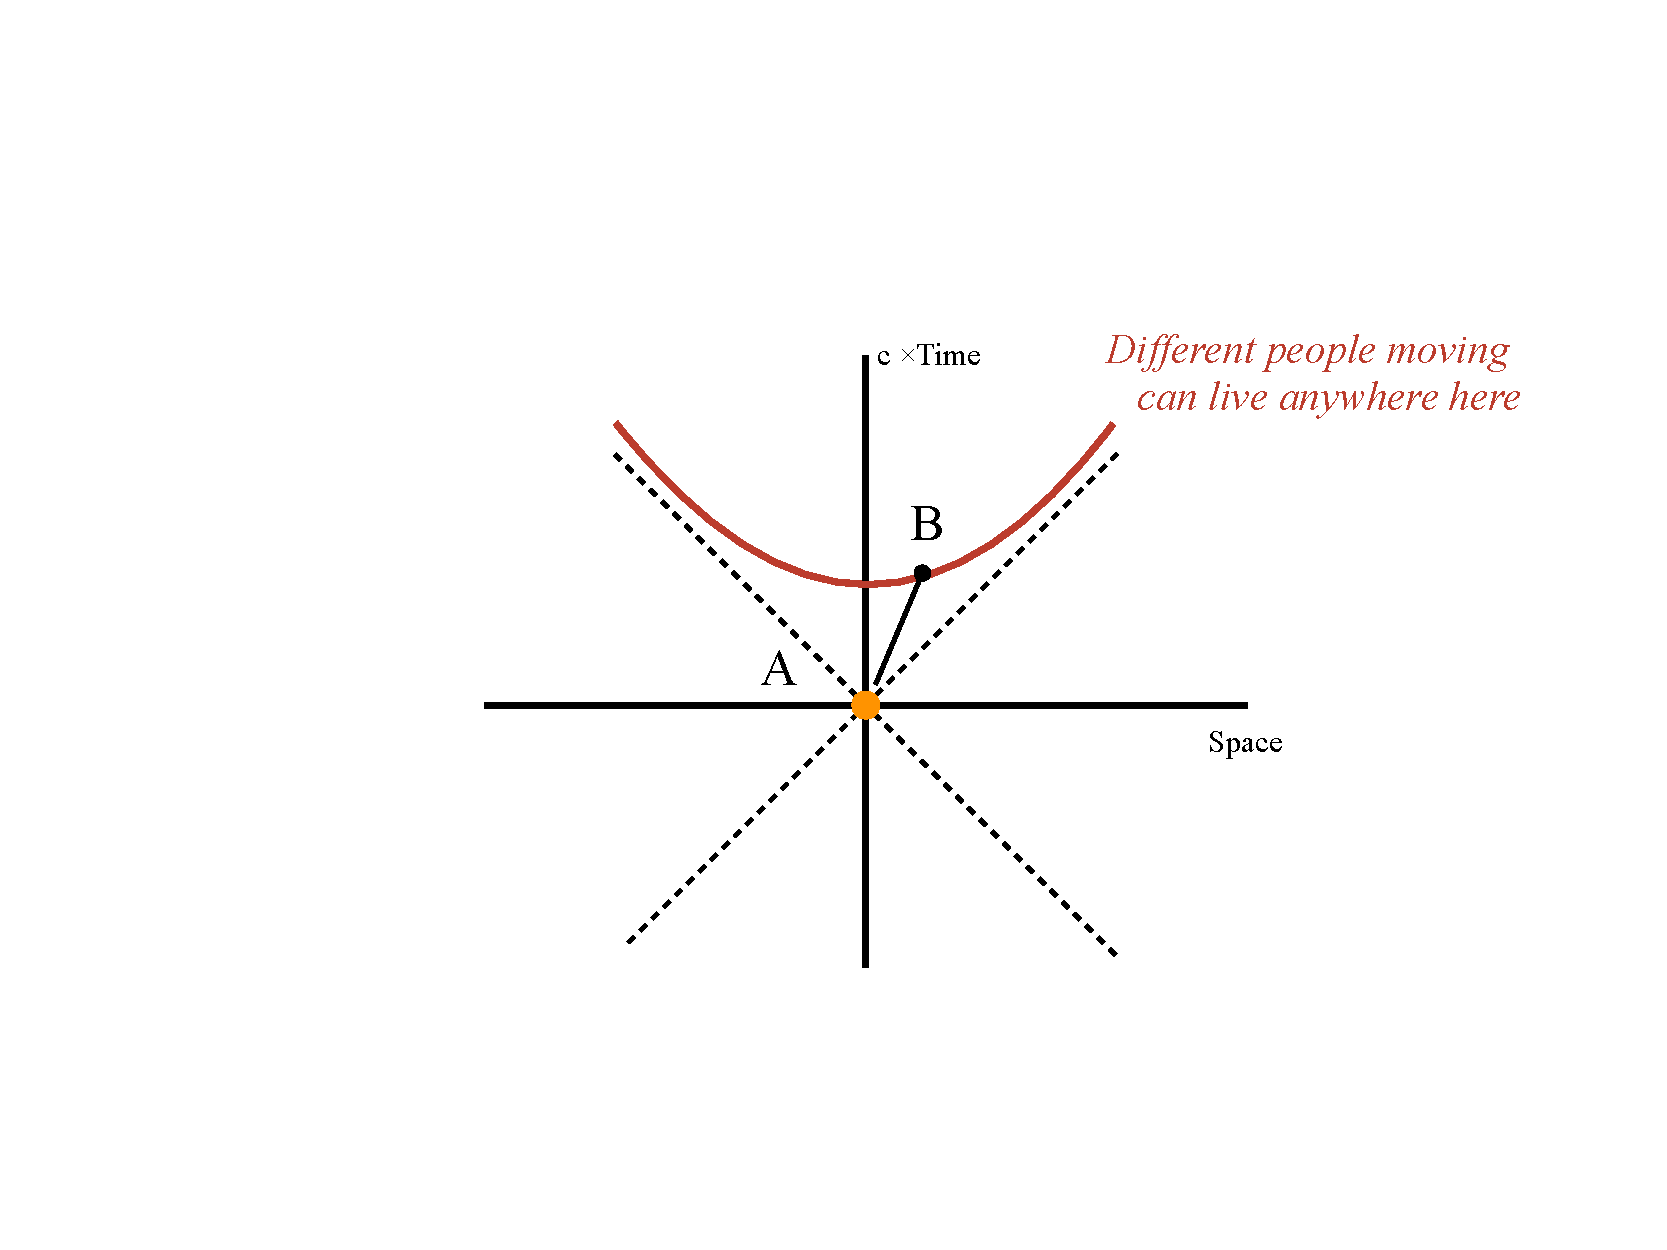
\includegraphics[width=0.6\textwidth]{./CausalityTimelike.pdf}
\end{figure}
All moving observers agree that A happens before B Can say safely say: ``A causes B''


However, If you could go faster than c, things go wrong...
\begin{figure}[h]
\centering
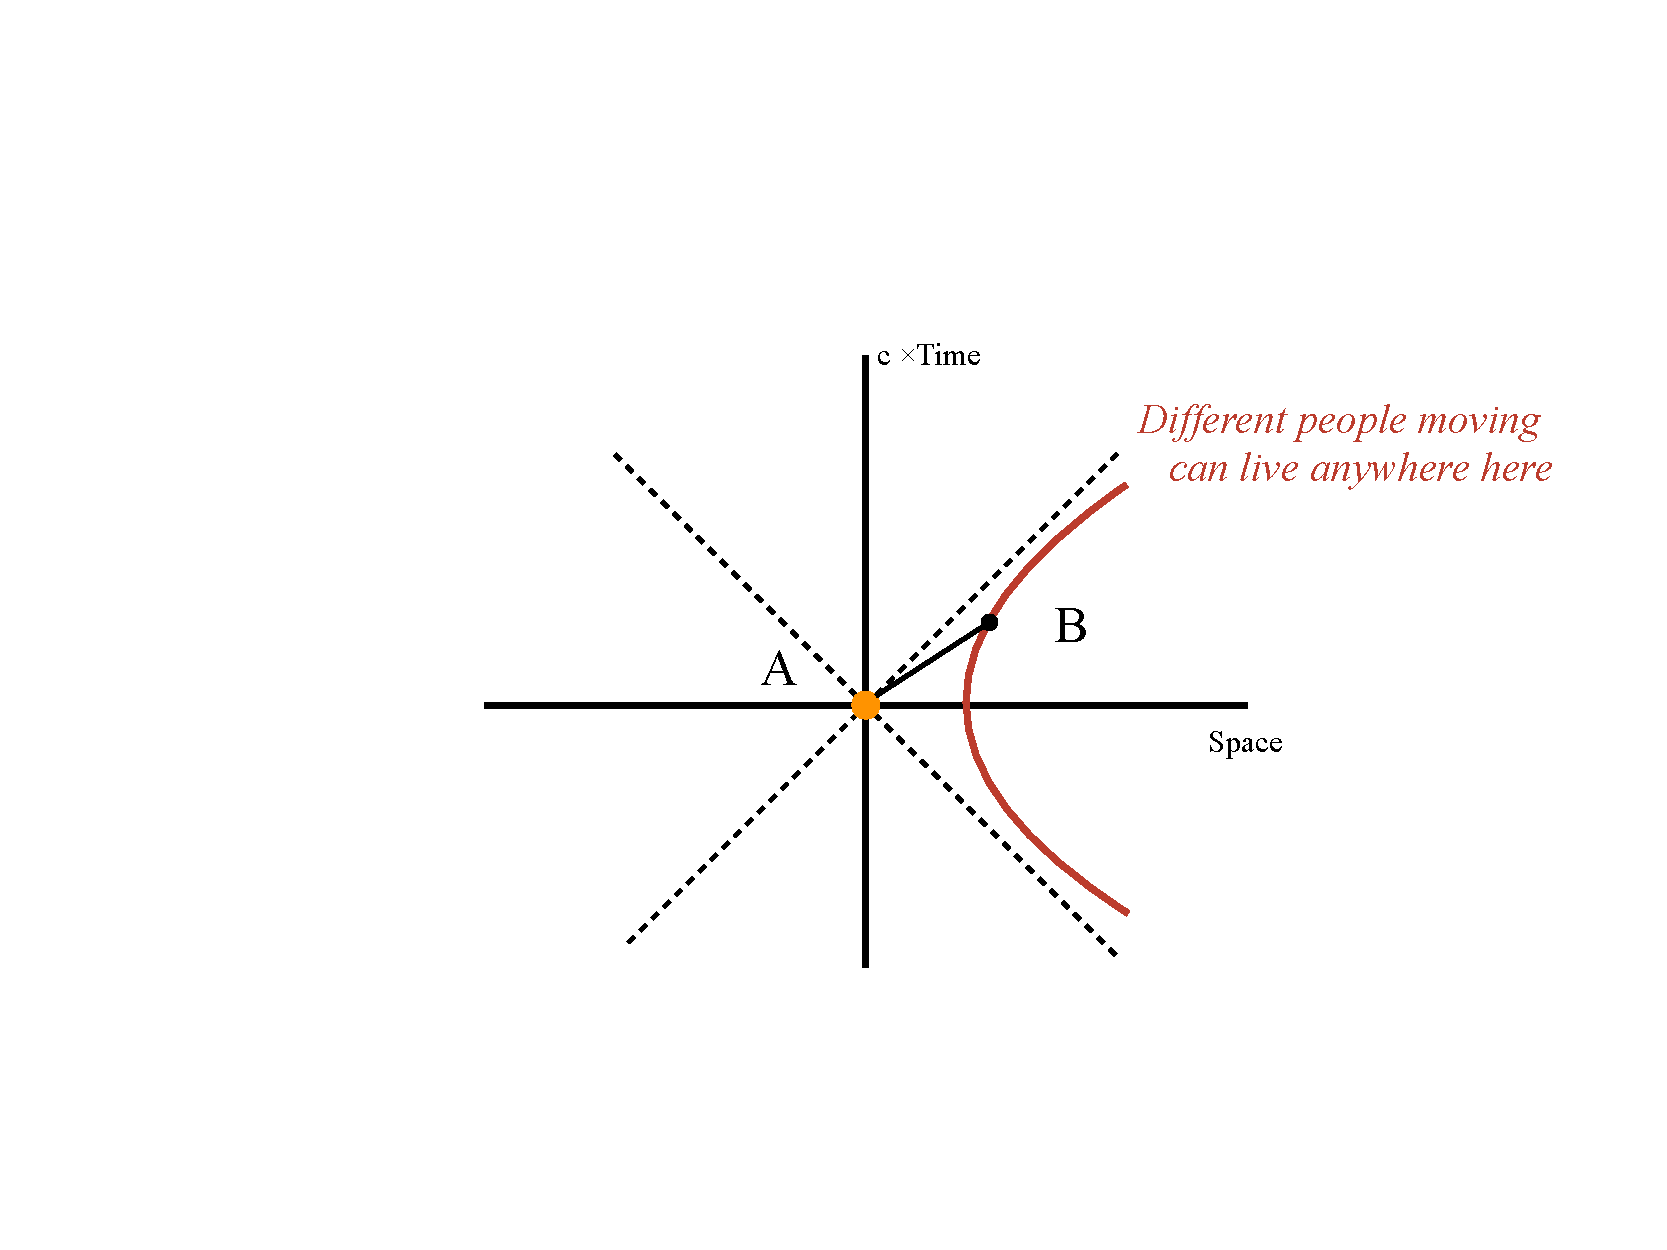
\includegraphics[width=0.6\textwidth]{./CausalitySpacelike.pdf}
\end{figure}
Depending about how you move, disagree about what comes first. Causality is violated. Bullet hits B before A pulls trigger.

Causality in Relativistic QM

w/QM always some non-zero probability of getting out.
Problem, looks like current is going backwards in time from A to B
Way out, if interpret this as B sending something to A
But B has to send something with opposite charge. (know A lost charge)


For the theory to have a prayer of being both quantum mechanical and relativisit there must exist particles that are identical to proton (say) except with opposite charge.
Anti-particles !

\section{Vacuum}
Anti-mater in turn has major an impact on nothing, ie the vacuum.

What does it take to study empty space (“the vacuum”) ?
Nothing special...until try to check small regions

\textbf{Before QM:}
Build tiny robots. (Get tiny robots to build tinier robots, who ..)

\textbf{With QM:}
At small distances, uncertainty principle kicks in
Need large $\Delta p$ (or equivalently large $\Delta E$)
Smaller and smaller distances, need higher and higher energies


Empty Space Interesting

When eventually get to small enough distances to need $\Delta E$ ~ 2$m_e c^2$
Nothing prevents creation of particle - anti-particle pair
- Everything is conserved (energy/charge/...) - Some probability for this to happen

Completely changes our picture of the vacuum
- Simple act of looking at the creates something - No sense in which the vacuum is empty

Often here accelerator as worlds most powerful microscopes
Looking at the vacuum


\section{Other Implications Combining SR \& QM}

\textbf{Spin}
QM: QM + R:
 Could accommodate spin
Any 1/2 integer value allowed
Forced to talk spin (Something special w/massless particles) Integer spin = Bosons / Half-integer = Fermions Can only have: 0 1/2 1 3/2 2
Interactions
QM: Any conceivable interaction possible
QM + R: Charge is conserved
Local (no more action at a distance)
Only finite number of specific interactions allowed :
\begin{figure}[h]
\centering
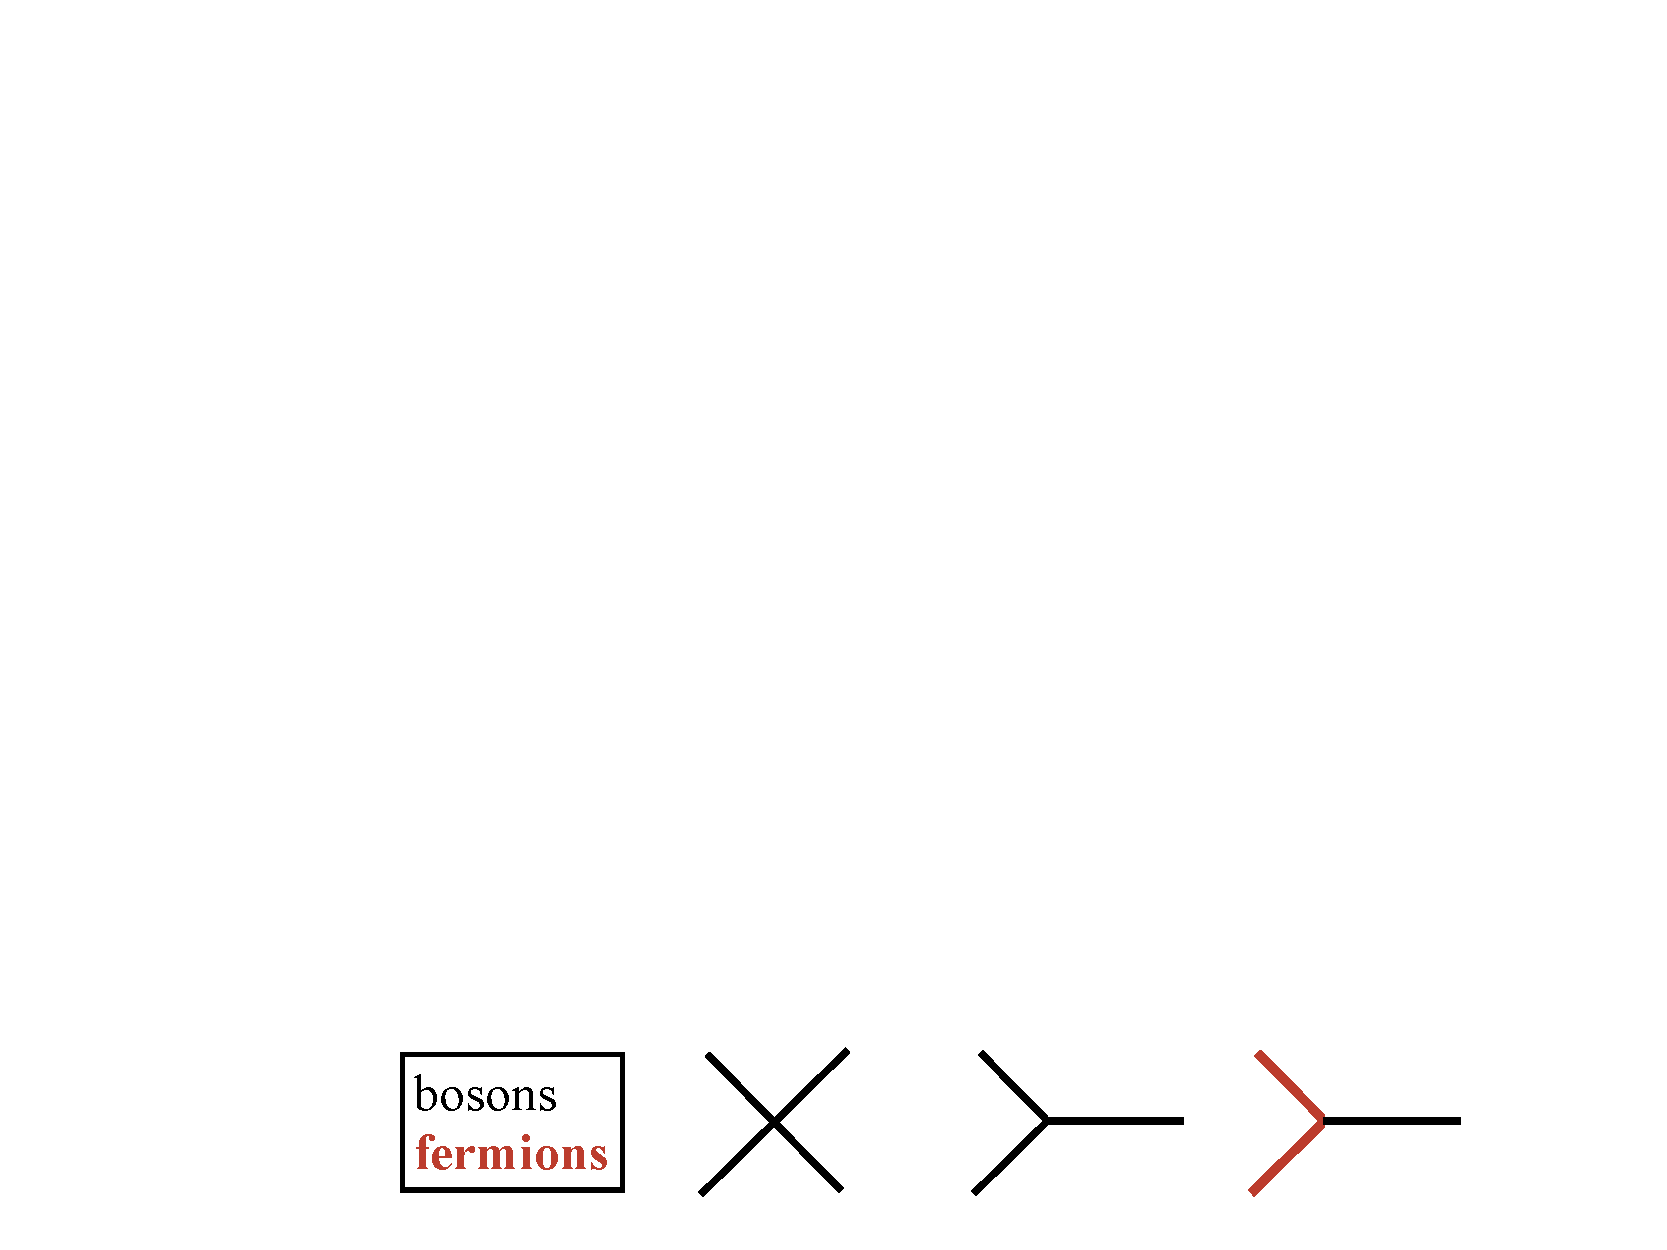
\includegraphics[width=0.6\textwidth]{./AllowedInteractions.pdf}
\end{figure}


In this course we will outline this basic framework for any possible theory.
And then talk about the particular version that we actually observe.


\end{document}


